\documentclass{article}
\usepackage{graphicx}
\usepackage{amsmath}
\usepackage{hyperref}
\usepackage{booktabs}
\usepackage{makeidx}
\usepackage{sectsty}
\usepackage{hyperref}
\usepackage{textcomp}
\usepackage{wrapfig} % For wrapping text around figures
\usepackage{etoolbox} % for \AtBeginDocument
\usepackage[margin=2]{geometry} % Set margin size to 2cm on all sides




\newgeometry{top=-1cm, bottom=2cm, left=1cm, right=1cm} % Set smaller margins for the first page only

\title{
    \begin{center}
     \hspace*{-2cm}
\includegraphics[width=1.25\textwidth]{Met_logo.png}\\
    \end{center}
    \vspace{1cm}
    \huge\textbf{Car Data Analysis Dashboard}\\
    \huge\textbf{Project Report}\\
    \vspace{1cm}
    \textbf{Seminar Report}\\
    \vspace{1cm}
    \fontsize{18}{15}\selectfont{Data Analysis with Python and PowerBI }\\
    \vspace{1cm}
    \fontsize{15}{15}\selectfont\textbf{BACHELOR OF TECHNOLOGY}\\
    \vspace{0.2cm}
    \fontsize{18}{15}\selectfont{Computer Science and Design }\\
    \vspace{0.2cm}
    \fontsize{18}{15}\selectfont\textbf{2023-24}\\
    \vspace{2cm}
    \fontsize{18}{15}\selectfont{Submitted by :}\\
    \vspace{0.5cm}
    \fontsize{15}{15}\selectfont\textbf{{MAYUR BORGUDE\vspace{0.3cm}\\RUSHIKESH SHINDE }}\\
    \vspace{1cm}
    \begin{center}
    
\includegraphics[width=0.2\textwidth]{batu_logo.jpg}\\
    \end{center}
    
}



\AtBeginDocument{\maketitle\newpage\restoregeometry}

\begin{document}
\newgeometry{margin=2cm}
.\\
\vspace{0cm}
    \begin{center}
    \fontsize{28}{15}\selectfont\textbf{CERTIFICATE}\\
    \vspace{2cm}
    \fontsize{18}{15}\selectfont{[Third Year B-Tech Computer Science and Design]}\\
    \vspace{0.2cm}
    \fontsize{18}{15}\selectfont{Semister - VI}\\
    \vspace{1.2cm}
    \fontsize{15}{15}\selectfont\textbf{MAYUR BORGUDE\vspace{0.3cm}\\RUSHIKESH SHINDE }\\
    \vspace{1.2cm}
    \fontsize{18}{15}\selectfont{Has Successfully Completed his Seminar on}\\
    \vspace{0.6cm}
    \fontsize{18}{15}\selectfont\textbf{"Car Data Analysis Dashboard"}\\
    \vspace{1cm}
    \fontsize{18}{15}\selectfont{Towards the Partial Fulfillment of Bachelor of Technology\newline [Computer Science and Design] }\\
    \vspace{1.5cm}
    \fontsize{18}{18}\selectfont\textbf{Dr. Babasaheb Ambedkar Technological}\\
    \fontsize{18}{18}\selectfont\textbf{University,Lonere}\\
    \vspace{0.2cm}
    \fontsize{18}{15}\selectfont{During the Academic}\\
    \vspace{0.1cm}
    \fontsize{18}{15}\selectfont{Year 2023-2024}\\
    \vspace{5cm}
    \end{center}

\begin{center}
    {\fontsize{15}{15}\selectfont
    \setlength{\tabcolsep}{13pt}
    \begin{tabular}{ccc} % 3 columns
        \textbf{Prof. G.V.Sonawane} & \textbf{Prof. S.S.Sheikh} & \textbf{Dr.Rajendra Narkhede} \\ % Row 1
        Seminar Guide & Head of Dept. & Principal  \\ % Row 2
    \end{tabular}
    }
\end{center}

\newpage

\tableofcontents


\newpage
\listoffigures
    

\newpage

\begin{abstract}

In the rapidly evolving landscape of the automotive industry, data analytics has emerged as a powerful tool for driving innovation, optimizing operations, and gaining competitive advantage. This abstract provides an overview of a comprehensive data analysis project aimed at leveraging technologies such as Python, R, Power BI, Kaggle, ETL (Extract, Transform, Load), OLAP (Online Analytical Processing), and OLTP (Online Transaction Processing) to analyze car data attributes and extract actionable insights for stakeholders in the automotive sector.
\\
The project encompasses a multifaceted approach to car data analysis, encompassing data collection, preprocessing, analysis, visualization, and interpretation. Leveraging Python and R programming languages, data from various sources, including Kaggle datasets and proprietary databases, are collected and processed using ETL techniques to ensure consistency, accuracy, and completeness.
\\
\\
The processed data is then analyzed using a combination of descriptive statistics, regression analysis, clustering, and predictive modeling techniques to uncover patterns, trends, and relationships within the car data attributes. Advanced analytics tasks such as price prediction, demand forecasting, and customer segmentation are performed to generate actionable insights for stakeholders.
\\
The visualization and exploration of car data attributes are facilitated through interactive dashboards and reports developed using Power BI. These dashboards provide users with intuitive tools for exploring and analyzing the data dynamically, enabling them to derive valuable insights into market trends, consumer preferences, and operational performance.
\\
\\
In addition to traditional data analysis techniques, the project also explores the use of OLAP and OLTP technologies to support complex querying and reporting requirements. OLAP cubes are utilized to aggregate and summarize car data across multiple dimensions, providing users with a multidimensional view of the data for deeper analysis. OLTP systems are employed to support real-time transaction processing and data updates, ensuring that users have access to the most up-to-date information.
\\
\\
The project aims to address a variety of challenges associated with car data analysis, including data integration, preprocessing, visualization, advanced analytics, and user adoption. By leveraging a combination of cutting-edge technologies and best practices, the project seeks to empower stakeholders in the automotive industry with the tools and insights necessary to make informed decisions, optimize operations, and drive business growth.
\\
\\
In conclusion, this abstract provides a high-level overview of a comprehensive data analysis project aimed at leveraging Python, R, Power BI, Kaggle, ETL, OLAP, and OLTP technologies to analyze car data attributes and extract actionable insights for stakeholders in the automotive industry. Through effective collaboration, innovative solutions, and a commitment to excellence, the project aims to overcome the challenges posed by car data analysis and unlock new opportunities for innovation and transformation in the automotive sector.

To facilitate user-friendly exploration and visualization of the analyzed data, interactive dashboards and reports are developed using Power BI. These dashboards offer intuitive interfaces with dynamic filtering and drill-down capabilities, empowering users to interactively explore and analyze the data. Additionally, the project explores the utilization of OLAP technology to provide multidimensional analysis capabilities, enabling users to slice and dice the data across multiple dimensions for deeper insights.
\\
\\
In addressing the challenges associated with car data analysis, such as data integration, preprocessing, visualization, and advanced analytics, the project aims to deliver a comprehensive solution that meets the diverse needs of stakeholders in the automotive industry. By leveraging cutting-edge technologies and adhering to best practices, the project strives to empower stakeholders with the tools and insights necessary to optimize operations, improve decision-making, and drive business growth.

In conclusion, this abstract provides a holistic overview of a sophisticated data analysis project that leverages Python, R, Power BI, Kaggle, ETL, OLAP, and OLTP technologies to analyze car data attributes. Through its multidisciplinary approach and commitment to excellence, the project aims to unlock new opportunities for innovation and transformation in the automotive sector, ultimately driving progress and competitiveness in an increasingly data-driven industry landscape.\\
\end{abstract}
\addcontentsline{toc}{section}{Abstract}
\index{Abstract}


\sectionfont{\huge\centering}
\subsectionfont{\Large}
\subsubsectionfont{\large}
\newpage
\section{Introduction}
\vspace{1cm}
{\fontsize{15}{15}\selectfont
In the dynamic landscape of the automotive industry, data has emerged as a transformative force, reshaping traditional paradigms and revolutionizing business strategies. Amidst evolving consumer preferences, technological advancements, and market dynamics, stakeholders across the automotive value chain are increasingly turning to data analytics as a means to gain a competitive edge and drive sustainable growth. The Car Data Analysis Dashboard project stands as a testament to this trend, offering a comprehensive platform for harnessing the power of data to inform decision-making, optimize operations, and unlock new opportunities for innovation.

The significance of the Car Data Analysis Dashboard project lies in its potential to address the myriad challenges facing the automotive industry in the digital age. From manufacturers seeking insights into emerging market trends and consumer preferences to dealerships optimizing inventory management and pricing strategies, the dashboard aims to cater to a diverse range of stakeholders with its robust analytics and intuitive visualization capabilities. By consolidating disparate data sources and providing a centralized platform for analysis, the dashboard empowers users with the tools necessary to navigate the complexities of the automotive landscape effectively.

\begin{figure}[htbp]
  \centering
  \vspace{0.3cm}
  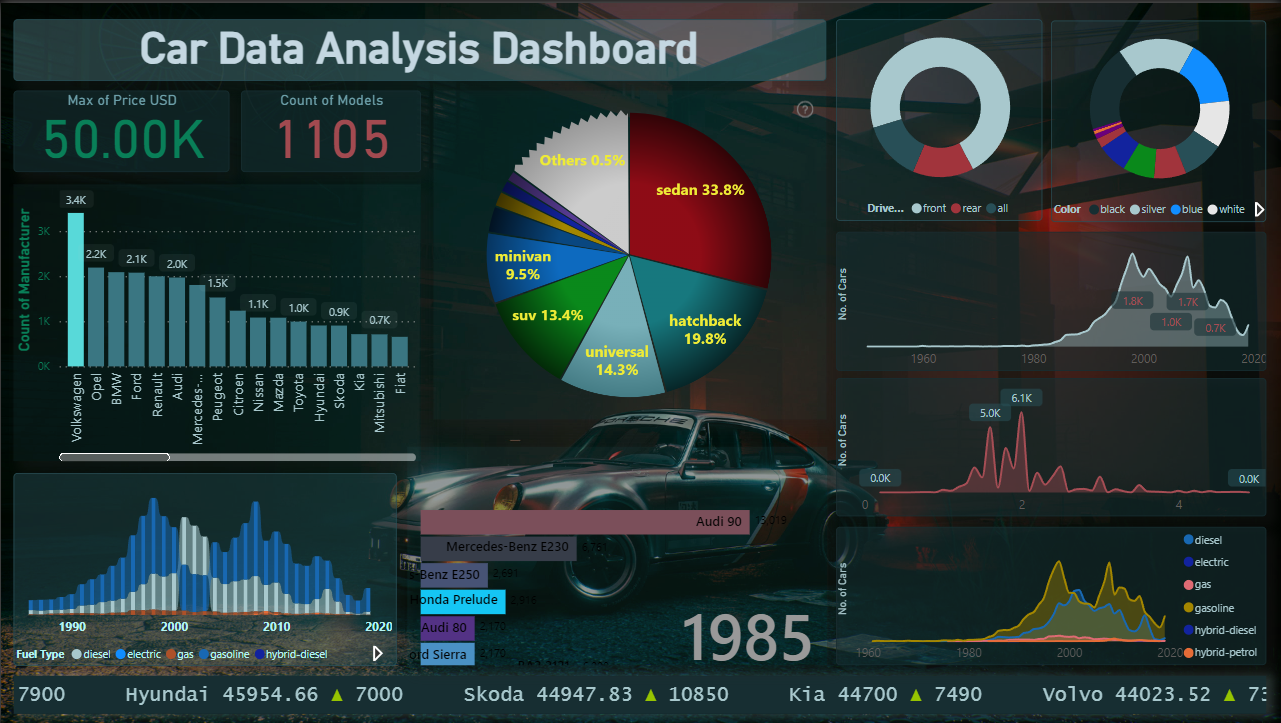
\includegraphics[width=0.7\textwidth]{Figures/dashboard1.png}\\
  \caption{Car Data Analysis Dashboard}
  \vspace{0.3cm}
\end{figure}

At its core, the Car Data Analysis Dashboard is designed to facilitate data-driven decision-making by providing stakeholders with actionable insights derived from a wealth of car-related attributes. Whether it's identifying trends in fuel efficiency, analyzing the impact of advanced features on pricing, or understanding regional variations in consumer preferences, the dashboard offers a multifaceted view of the automotive market, enabling users to make informed choices and capitalize on emerging opportunities.
\newline
Moreover, the project holds implications beyond immediate business objectives, extending to broader societal concerns such as sustainability and innovation. By analyzing trends in fuel types, engine capacities, and emissions standards, the dashboard can inform discussions around environmental impact and drive efforts towards greener, more sustainable transportation solutions. Furthermore, by identifying patterns in consumer behavior and market demand, the project lays the groundwork for future research and innovation, guiding the development of next-generation vehicles that align with evolving societal needs and preferences.
\newline
\newline
In this academic report, we delve into the intricacies of the Car Data Analysis Dashboard project, offering insights into its inception, development methodology, and anticipated outcomes. Through a combination of rigorous data preprocessing, advanced analytics, and user-centric design principles, the dashboard seeks to empower stakeholders with the knowledge and insights necessary to navigate the complexities of the automotive landscape effectively. As we embark on this journey, it is our hope that this report will serve as a valuable resource for industry professionals, researchers, and policymakers alike, shedding light on the transformative potential of data-driven solutions in shaping the future of mobility.
\newline
\newline
The automotive industry, a cornerstone of modern civilization, has always been at the forefront of technological innovation. In recent years, the advent of big data and advanced analytics has revolutionized the way automotive companies operate, enabling them to extract actionable insights from vast amounts of data and gain a competitive edge in an increasingly complex and competitive market. This literature review aims to explore the evolving role of data analytics in the automotive industry, with a focus on its applications, challenges, and future prospects.
}
\index{Introduction}


\newpage
\section{Problem Statement}
\vspace{1cm}
{\fontsize{15}{15}\selectfont

Introduction:

The automotive industry is undergoing a profound transformation driven by technological advancements, changing consumer preferences, and evolving market dynamics. In this rapidly evolving landscape, automotive companies are increasingly turning to data analytics as a means to gain insights, optimize operations, and stay ahead of the competition. The problem at hand revolves around the need to develop a comprehensive data analysis solution leveraging Power BI and Python programming for analyzing car data attributes including Name, Manufacturer, Model, Transmission, Color, Odometer value, Production Year, Fuel Type, Gas Availability, Engine Capacity, Body Type, Status, DriveTrain, Advanced Features, and Price USD.

\subsection{Problem Definition:}

The primary objective of this project is to develop a robust data analysis solution that enables stakeholders in the automotive industry to extract actionable insights from a diverse range of car data attributes. The solution should encompass both data preprocessing and analysis components, leveraging the capabilities of Power BI for interactive visualization and Python programming for advanced analytics. The specific challenges addressed by this project include:

\subsection{Data Integration and Preprocessing:}

Challenge: The car data may be sourced from disparate datasets with varying formats, structures, and quality levels. Integrating and preprocessing this data to ensure consistency, accuracy, and completeness is a critical challenge.
\\
Solution: Develop data preprocessing pipelines using Python programming to handle tasks such as data cleaning, normalization, imputation of missing values, and standardization of data formats. Ensure compatibility with Power BI for seamless integration into the visualization dashboard.

\subsection{Interactive Visualization and Exploration:}

Challenge: Automotive stakeholders require intuitive and interactive visualization tools to explore and analyze car data attributes effectively. Static reports or traditional spreadsheet-based analyses may not suffice in providing actionable insights.
\\
Solution: Utilize Power BI's rich visualization capabilities to create interactive dashboards and reports that enable users to explore car data attributes dynamically. Incorporate features such as filters, slicers, and drill-down functionality to facilitate deeper insights and exploration.

\subsecction{Advanced Analytics and Insights Generation:}

Challenge: Extracting meaningful insights from car data attributes requires advanced analytics techniques such as descriptive statistics, regression analysis, clustering, and predictive modeling. Implementing these techniques in a scalable and efficient manner presents a significant challenge.
\\
Solution: Leverage Python programming libraries such as Pandas, NumPy, and Scikit-learn to perform advanced analytics and machine learning tasks on the car data. Develop models for price prediction, demand forecasting, and customer segmentation to generate actionable insights for stakeholders.


\subsection{Performance and Scalability:}

Challenge: As the volume and complexity of car data increase, the performance and scalability of the data analysis solution become paramount. The solution must be capable of handling large datasets efficiently and scaling to meet growing demands.
\\
Solution: Optimize data processing pipelines and algorithms using parallel processing, distributed computing, and other techniques to improve performance and scalability. Leverage cloud-based services such as Azure or AWS for scalable storage and compute resources.

}

\index{Problem Statement}



\newpage
\section{Literature Review}
\vspace{1cm}
{\fontsize{15}{15}\selectfont


The automotive industry, a cornerstone of modern civilization, has always been at the forefront of technological innovation. In recent years, the advent of big data and advanced analytics has revolutionized the way automotive companies operate, enabling them to extract actionable insights from vast amounts of data and gain a competitive edge in an increasingly complex and competitive market. This literature review aims to explore the evolving role of data analytics in the automotive industry, with a focus on its applications, challenges, and future prospects.

\subsection{Applications of Data Analytics in the Automotive Industry:}

Data analytics has permeated every aspect of the automotive industry, from product development and manufacturing to marketing and customer service. One of the primary applications of data analytics in the automotive sector is predictive maintenance, where machine learning algorithms are used to analyze vehicle sensor data and predict potential failures before they occur. By proactively addressing maintenance issues, automotive companies can reduce downtime, minimize repair costs, and improve overall operational efficiency.

Another key application of data analytics in the automotive industry is in the realm of marketing and sales. With the proliferation of digital channels and the rise of e-commerce, automotive companies are leveraging data analytics to better understand customer behavior, segment their target audience, and personalize marketing campaigns. By analyzing data from sources such as social media, website traffic, and customer transactions, companies can identify trends, preferences, and purchase intent, enabling them to tailor their marketing efforts for maximum impact.

Data analytics is also playing an increasingly important role in vehicle design and development. By analyzing data from sources such as customer feedback, vehicle performance tests, and simulated driving scenarios, automotive engineers can gain valuable insights into how different design features and configurations impact vehicle performance, safety, and comfort. This data-driven approach to design not only enables companies to create more innovative and competitive products but also helps them optimize the design process and reduce time-to-market.

\subsection{Challenges and Limitations:}

Despite its potential benefits, the widespread adoption of data analytics in the automotive industry is not without its challenges. One of the primary challenges facing automotive companies is the sheer volume and complexity of data generated by modern vehicles. With the advent of connected cars and autonomous driving technologies, vehicles are generating massive amounts of data every second, presenting significant challenges in terms of data storage, processing, and analysis.

Another challenge facing automotive companies is data privacy and security. With the increasing digitization of vehicles and the growing interconnectedness of automotive systems, concerns about data privacy and security have become more pronounced. Automotive companies must ensure that they have robust data protection measures in place to safeguard sensitive customer information and comply with regulations such as the General Data Protection Regulation (GDPR) and the California Consumer Privacy Act (CCPA).

Furthermore, there are challenges related to data quality and accuracy. Automotive data is often heterogeneous and fragmented, coming from a wide range of sources such as vehicle sensors, telematics systems, and third-party vendors. Ensuring the quality and accuracy of this data is essential for generating reliable insights and making informed decisions. However, achieving data quality and accuracy can be challenging, especially when dealing with data from disparate sources and formats.

\subsection{Future Prospects:}

Looking ahead, the future of data analytics in the automotive industry appears promising, with continued advancements in technology and analytics capabilities. One area of particular interest is the use of artificial intelligence (AI) and machine learning (ML) algorithms to extract insights from complex and unstructured data sources. By leveraging AI and ML, automotive companies can gain deeper insights into customer behavior, market trends, and vehicle performance, enabling them to make more informed decisions and stay ahead of the competition.

Another area of future growth is the integration of data analytics with emerging technologies such as the Internet of Things (IoT) and blockchain. With the proliferation of connected cars and IoT devices, automotive companies have access to unprecedented amounts of real-time data about vehicle performance, driver behavior, and environmental conditions. By integrating data analytics with IoT platforms, companies can gain actionable insights in real-time, enabling them to optimize vehicle operations, improve safety, and enhance the overall customer experience.


}

\index{Literature Review}

\newpage
\section{Methodology}
\vspace{1cm}
{\fontsize{15}{15}\selectfont

\subsection{Process of Dashboard Creation}

\subsubsection{Data Collection:}

Identify and access relevant datasets containing car data attributes such as Name, Manufacturer, Model, Transmission, Color, Odometer value, Production Year, Fuel Type, Gas Availability, Engine Capacity, Body Type, Status, DriveTrain, Advanced Features, and Price USD.
Utilize Kaggle, publicly available datasets, and proprietary sources to collect comprehensive data.
\subsubsection{Data Preprocessing:}

Perform data cleaning to handle missing values, outliers, and inconsistencies.
Normalize and standardize data formats for consistency.
Convert categorical variables into numerical representations using techniques like one-hot encoding or label encoding.
Handle data imbalances and skewness through techniques such as oversampling, undersampling, or data transformation.
Split the dataset into training and testing sets for model evaluation.
\subsubsection{Exploratory Data Analysis (EDA):}

Conduct exploratory data analysis to gain insights into the distribution and characteristics of car data attributes.
Visualize key attributes using histograms, scatter plots, box plots, and correlation matrices to identify patterns, trends, and relationships.
Perform statistical analysis to calculate summary statistics, identify outliers, and detect anomalies.
\begin{figure}[htbp]
  \centering
  \vspace{0.3cm}
  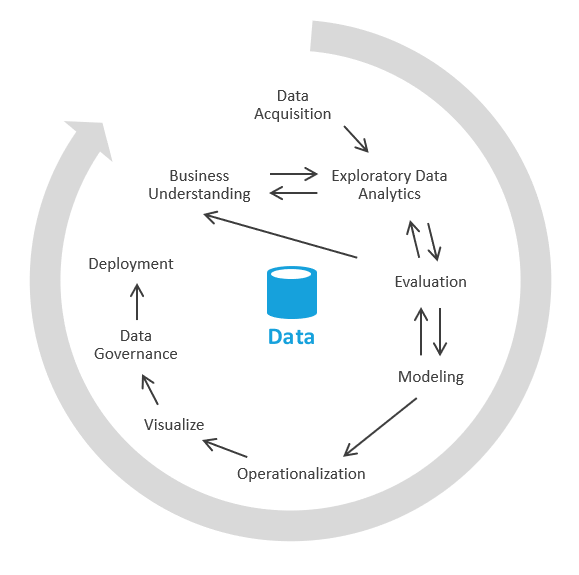
\includegraphics[width=0.6\textwidth]{Figures/Python/EDA.png}\\
  \caption{Data Analysis Lifecycle}
  \vspace{0.3cm}
\end{figure}
\\
\subsubsection{Feature Engineering:}

Engineer new features based on domain knowledge and insights gained from EDA.
Create interaction terms, polynomial features, or transformations to capture nonlinear relationships.
Select relevant features using techniques such as feature importance, correlation analysis, or domain expertise.
\subsubsection{Model Development:}

Select appropriate machine learning models based on the nature of the problem (e.g., regression for price prediction, classification for status prediction).
Train the selected models using the training dataset and evaluate their performance using cross-validation techniques such as k-fold validation.
Tune hyperparameters to optimize model performance and prevent overfitting using techniques such as grid search or random search.
Compare the performance of different models based on evaluation metrics such as mean squared error (MSE), mean absolute error (MAE), accuracy, precision, recall, and F1-score.
\subsubsection{Dashboard Development:}

Utilize Power BI for developing interactive dashboards and reports.
Integrate processed data into Power BI and create visualizations such as bar charts, line graphs, scatter plots, and heatmaps to present key insights.
Implement interactive features such as filters, slicers, and drill-down functionality to enable users to explore and analyze the data dynamically.
Design the dashboard interface for usability, intuitiveness, and accessibility across different devices and screen sizes.
\subsubsection{Deployment and Maintenance:}

Deploy the developed dashboard to the intended users or stakeholders within the organization.
Provide user training and support to ensure effective adoption and utilization of the dashboard.
Monitor the performance and usage of the dashboard over time and incorporate feedback from users to make iterative improvements.
Update the dashboard periodically with new data and insights to ensure relevance and accuracy.
\subsubsection{Documentation and Reporting:}

Document the entire methodology, including data sources, preprocessing steps, model development process, and dashboard design considerations.
Prepare comprehensive reports summarizing key findings, insights, and recommendations derived from the analysis.
Share the reports and documentation with stakeholders to facilitate informed decision-making and drive actionable outcomes.


\subsection{Tools and thier Application}

\subsubsection{ Kaggle (Data Acquisition)}

\href{https://www.kaggle.com/}{Kaggle}., a renowned platform for data science competitions and datasets, offers a plethora of datasets relevant to the automotive industry. The initial step in our methodology involves thorough exploration and evaluation of Kaggle's dataset repository to identify datasets aligning with our research objectives. Datasets covering a wide range of attributes such as car specifications, sales data, consumer reviews, and sentiment analysis are considered.

Upon identification of a suitable dataset, meticulous scrutiny is conducted to assess its quality, relevance, and completeness. Attributes crucial for our analysis, including car names, manufacturers, models, transmission types, colors, odometer values, production years, fuel types, engine capacities, and prices, are evaluated. Additionally, datasets accompanied by metadata or data dictionaries are preferred, as they provide valuable insights into the structure and semantics of the data.

After careful selection, the chosen dataset is acquired from Kaggle in a suitable format, typically CSV (Comma-Separated Values) or Excel. This format ensures compatibility and ease of integration with subsequent data analysis and preprocessing steps.

In the quest to acquire comprehensive car data for analysis, leveraging Kaggle proved to be a fruitful endeavor. Kaggle, a renowned platform for data science enthusiasts and professionals alike, hosts a plethora of datasets spanning diverse domains, including the automotive sector. Through diligent exploration and targeted search queries, a suitable dataset containing an extensive array of car attributes was identified. This dataset, sourced from reputable contributors and meticulously curated, offered a rich repository of information encompassing crucial details such as car names, manufacturers, models, transmission types, colors, production years, and more. Leveraging Kaggle's user-friendly interface and robust search functionalities facilitated efficient navigation and discovery, ensuring the acquisition of high-quality data for subsequent analysis. Overall, the utilization of Kaggle as a primary resource for accessing car data exemplified the platform's value in enabling data-driven insights and fostering collaborative exploration within the data science community.

the data is currently on \href{https://raw.githubusercontent.com/Mayborg121/Car_DataAnalysis_Dashboard/main/Car%20Dashboard/src/Raw/cars_data_raw.csv}{GitHub} : \href{https://github.com/Mayborg121/Car_DataAnalysis_Dashboard}{On My Profile (Mayborg121)}
\subsubsection{ Python (Data Cleaning and Preprocessing)}

Python emerges as a versatile and powerful tool for data cleaning and preprocessing, leveraging its rich ecosystem of libraries and intuitive syntax. The data cleaning and preprocessing pipeline encompasses several essential steps
\begin{figure}[htbp]
  \centering
  \vspace{0.3cm}
  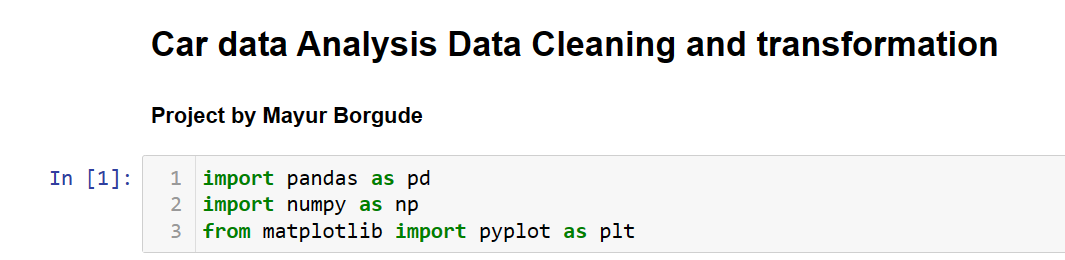
\includegraphics[width=1\textwidth]{Figures/Python/importing python libs.png}\\
  \caption{Importing Python Libraries}
  \vspace{0.3cm}
\end{figure}
\\
Importing data into pandas:
\\
Importing data into pandas is a fundamental step in data analysis and manipulation within Python. Using the 
"read\usepackage{textcomp}csv()"
function from the pandas library, CSV files can be effortlessly imported. By providing the file path as an argument, pandas intelligently reads the CSV data into a DataFrame—a tabular data structure. This DataFrame serves as the foundation for subsequent analysis, offering a wide array of functionalities for data exploration, transformation, and visualization. With its intuitive interface and powerful capabilities, pandas simplifies the process of importing data, facilitating seamless integration into Python-based data analysis workflows.
\\
\begin{figure}[htbp]
  \centering
  \vspace{0.3cm}
  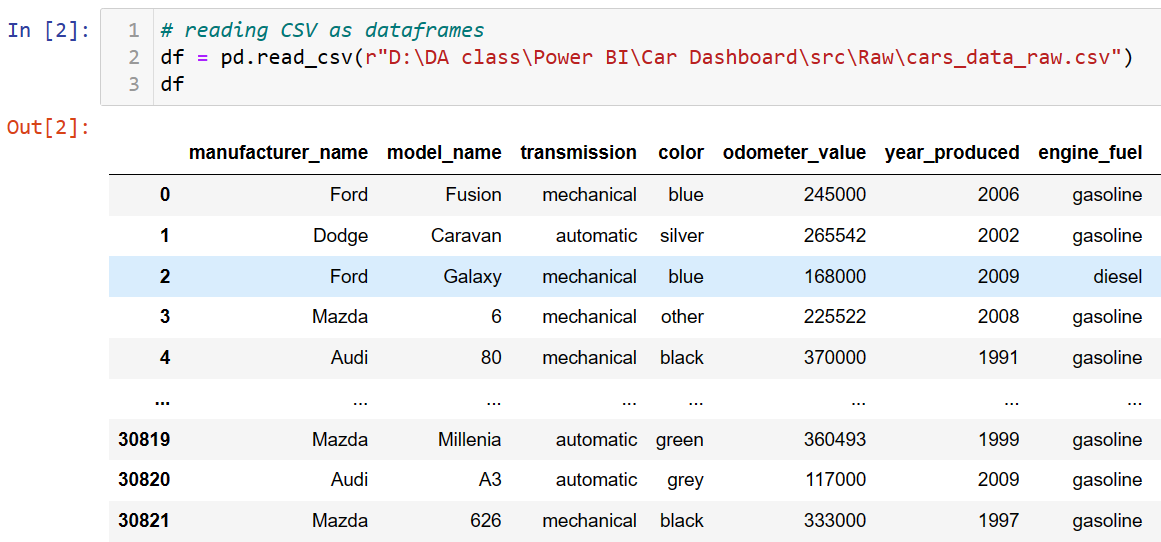
\includegraphics[width=0.8\textwidth]{Figures/Python/reading the data from CSV.png}\\
  \caption{Importing CSV datasets}
  \vspace{0.3cm}
\end{figure}
\\
\newpage
Data Cleaning:
\\
Handling Missing Values: Utilizing the Pandas library, missing values within the dataset are identified and addressed through techniques such as imputation or deletion. Imputation involves inferring missing values based on statistical measures such as mean, median, or mode, ensuring minimal disruption to the dataset's integrity.
Removing Duplicates: Duplicate entries, if any, are identified and eliminated to uphold data consistency and accuracy.
Correcting Data Inconsistencies: Inconsistent data values, including typos, formatting errors, or outliers, are rectified to maintain data quality and coherence.
\begin{figure}[htbp]
  \centering
  \vspace{0.3cm}
  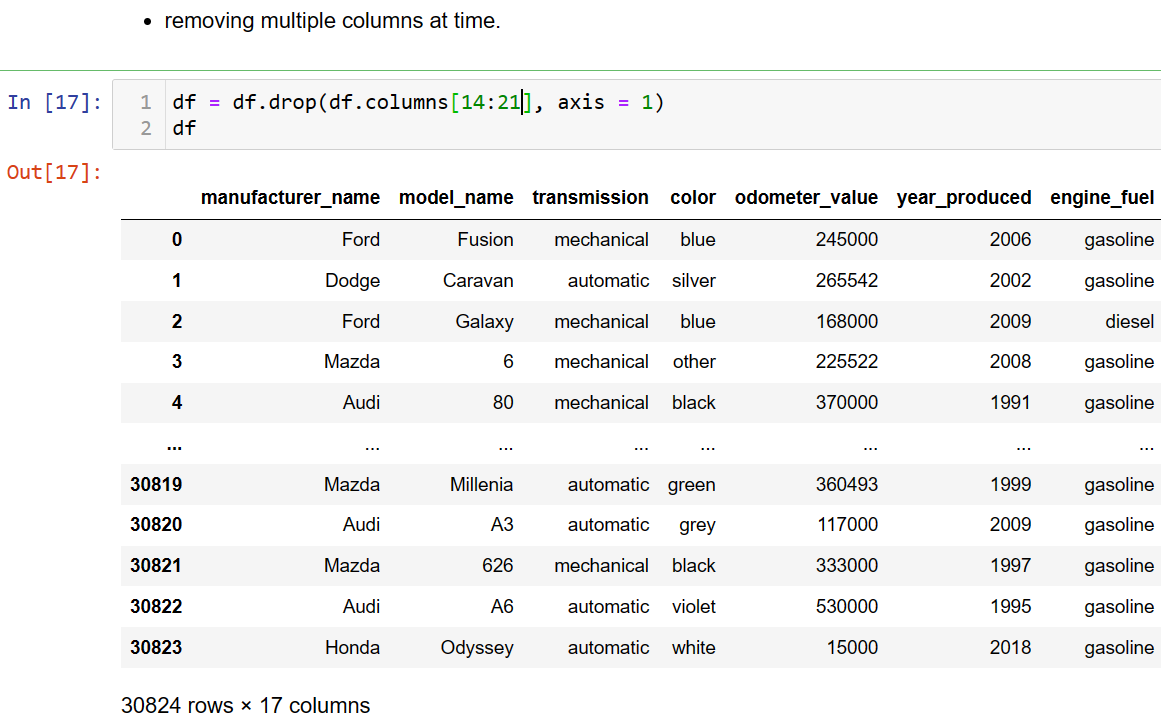
\includegraphics[width=1\textwidth]{Figures/Python/removing multiple columns.png}\\
  \caption{Removing irrelevant data}
  \vspace{0.3cm}
\end{figure}

\\
\\
Checking Null Values:
\\
Python scripts employing Pandas' functionalities, such as isnull() and sum(), are utilized to ascertain the presence of null values within each attribute of the dataset. This comprehensive assessment enables thorough understanding of data completeness and guides subsequent preprocessing decisions.
Deleting Irrelevant Data:

Non-essential or redundant columns within the dataset, which do not contribute meaningfully to the analysis objectives, are identified and removed. This streamlined approach ensures a focused dataset tailored to pertinent attributes, facilitating more targeted analysis.
\begin{figure}[htbp]
  \centering
  \vspace{0.3cm}
  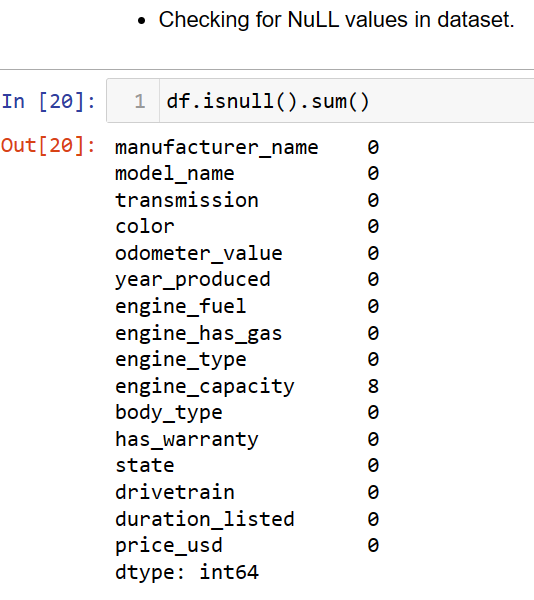
\includegraphics[width=0.5\textwidth]{Figures/Python/checking for null values.png}\\
  \caption{Checking For Null Values}
  \vspace{0.3cm}
\end{figure}
\\
\\
\\
Exporting the CSV:
\\
Upon completion of data cleaning and preprocessing, the refined dataset is exported to a new CSV file. This file serves as the foundation for subsequent analysis and visualization tasks within Power BI, ensuring seamless integration and continuity across the data analysis pipeline.
\begin{figure}[htbp]
  \centering
  \vspace{0.3cm}
  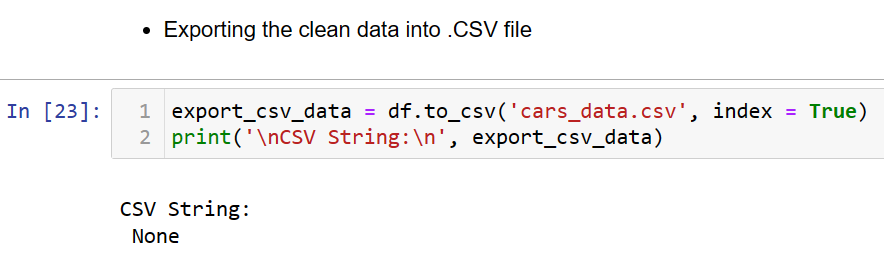
\includegraphics[width=1\textwidth]{Figures/Python/Exporting csv.png}\\
  \caption{Exporting Cleaned Dataset to CSV file}
  \vspace{0.3cm}
\end{figure}
\\
\\
\newpage
\subsubsection{Power BI (Data Analysis and Visualization)}

Power BI emerges as an indispensable tool for data analysis and visualization, offering intuitive interfaces and robust capabilities for exploring and presenting insights derived from the car data attributes. The methodology for data analysis and visualization in Power BI encompasses the following stages:
\\
\begin{figure}[htbp]
  \centering
  \vspace{0.3cm}
  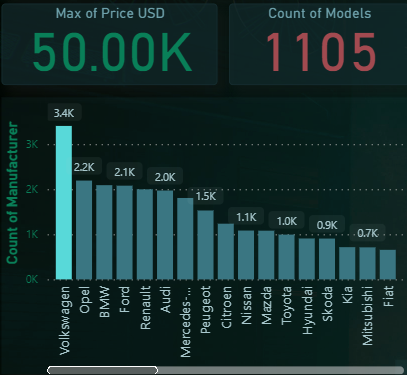
\includegraphics[width=0.6\textwidth]{Figures/PowerBI/infographics.png}\\
  \caption{Visualizations}
  \vspace{0.3cm}
\end{figure}
\\
Data Import:
\\
The cleaned and preprocessed dataset is imported into Power BI from the exported CSV file. Power BI's seamless integration with various data sources facilitates effortless data importation, ensuring accessibility and usability of the dataset within the Power BI environment.
\\
\\
Data Modeling:
\\
Power BI's advanced data modeling capabilities are harnessed to establish relationships between different tables within the dataset. These relationships are based on common attributes such as manufacturer names or model IDs, enabling seamless integration and analysis across disparate data sources.
\\
\\
Data Analysis:
\\
Power BI's native analytics features, including measures, calculated columns, and DAX (Data Analysis Expressions) functions, are leveraged to perform a myriad of analytical tasks. Descriptive statistics, such as counts, sums, averages, and percentages, are computed to derive insights into key metrics such as sales volume, average prices, and market share.
\\
\\
Visualization:
\\
A diverse array of visualization options available within Power BI, including bar charts, line charts, scatter plots, histograms, and pie charts, among others, are employed to represent the analyzed data. The selection of visualization types is driven by the nature of the data and the insights being communicated. For instance, bar charts may be utilized to compare sales performance across different manufacturers, while line charts may be preferred for visualizing trends in car prices over time.
The incorporation of interactive features such as filters, slicers, and drill-down capabilities enhances the usability of the visualizations, empowering users to explore the data dynamically and derive deeper insights.
\\
\\
Dashboard Creation:
\\
Power BI facilitates the creation of interactive dashboards by amalgamating multiple visualizations into a cohesive canvas. These dashboards provide a holistic view of key metrics and trends, enabling stakeholders to monitor performance and make data-driven decisions effectively.
}
\index{Methodology}




\newpage
\section{Data Analysis}
\vspace{1cm}
{\fontsize{15}{15}\selectfont

In today's data-driven world, the ability to analyze and derive insights from vast amounts of data is essential for informed decision-making and strategic planning. Python has emerged as a preferred choice among data analysts and scientists due to its rich ecosystem of libraries tailored for data manipulation, visualization, and analysis. Among these libraries, Pandas, Matplotlib, and Seaborn stand out as powerful tools for conducting data analysis and visualization. This note aims to explore the capabilities of these libraries and demonstrate their utility in performing data analysis tasks.

\subsection{Data Analysis Using Pandas}

Pandas is a versatile and powerful library for data manipulation and analysis in Python. At its core is the DataFrame, a tabular data structure similar to a spreadsheet, which allows for easy handling and manipulation of structured data.
Key features of Pandas include data ingestion from various sources such as CSV, Excel, SQL databases, and JSON; data cleaning and preprocessing; data manipulation through filtering, sorting, grouping, and aggregation; and data visualization and analysis.
Pandas provides intuitive and expressive syntax for performing complex data operations, making it an indispensable tool for data analysts and scientists.
Data Ingestion and Preprocessing with Pandas:

One of the first steps in data analysis is data ingestion, where data is loaded into memory from external sources. Pandas simplifies this process with functions like read\textunderscorecsv(), read\textunderscoreexcel(), read\textunderscoresql(), and more, allowing for seamless integration of data from diverse sources.
Once data is loaded, preprocessing steps such as handling missing values, removing duplicates, and converting data types may be necessary. Pandas provides methods like dropna(), fillna(), drop\textunderscoreduplicates(), and astype() for performing these tasks efficiently.

\subsection{Exploratory Data Analysis (EDA) with Pandas:}

Exploratory Data Analysis is a critical step in understanding the underlying patterns and characteristics of the data. Pandas offers a rich set of functionalities for conducting EDA, including summary statistics, data visualization, and correlation analysis.
Descriptive statistics such as mean, median, standard deviation, and quantiles can be computed using methods like describe() and mean(). Visualizations such as histograms, box plots, and scatter plots can be generated using Pandas' integration with Matplotlib and Seaborn.

\subsection{Data Visualization with Matplotlib and Seaborn:}

Matplotlib is a widely-used plotting library in Python, offering a wide range of plotting functions and customization options. Seaborn, built on top of Matplotlib, provides a high-level interface for creating attractive statistical visualizations.
Matplotlib allows for the creation of various types of plots, including line plots, bar plots, scatter plots, histograms, and more. Its object-oriented API offers fine-grained control over plot elements such as axes, labels, and legends.
Seaborn specializes in statistical data visualization, offering functions for visualizing relationships between variables, distribution of data, and categorical data. Its integration with Pandas DataFrames enables seamless plotting of data directly from DataFrame objects.

\begin{figure}[htbp]
  \centering
  \vspace{0.3cm}
  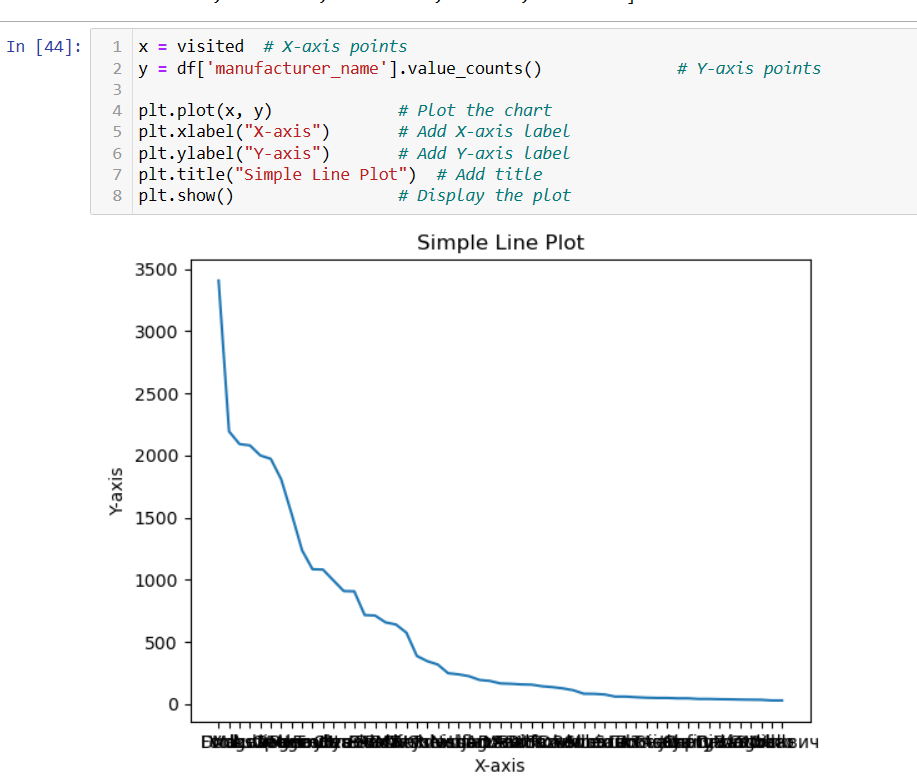
\includegraphics[width=0.8\textwidth]{Figures/Python/pythn analysis using matplotlib.png}\\
  \caption{Line chart using Matplotlib}
  \vspace{0.3cm}
\end{figure}

\newpage
\subsection{Advanced Data Analysis with Pandas:}

Pandas offers advanced functionalities for data manipulation and analysis, including data merging, reshaping, and time series analysis. Methods like merge(), pivot\textunderscore table(), and resample() facilitate complex data transformations and aggregations.
Additionally, Pandas provides support for handling time series data, including date/time indexing, resampling, and rolling window operations. This makes it suitable for analyzing temporal data such as stock prices, sensor readings, and economic indicators.
\\
\begin{figure}[htbp]
  \centering
  \vspace{0.3cm}
  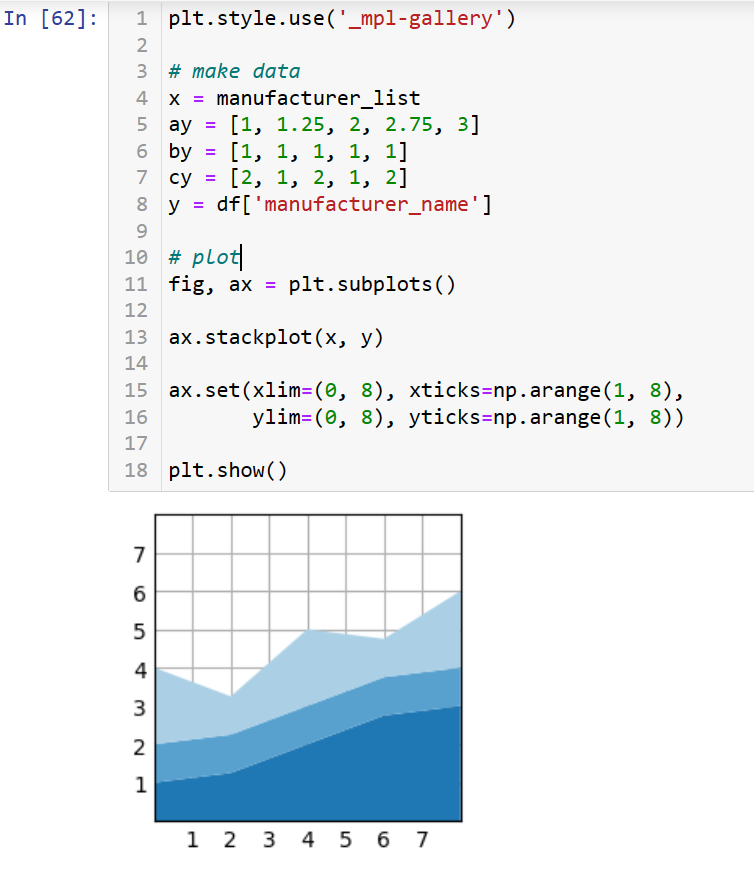
\includegraphics[width=0.8\textwidth]{Figures/Python/analysis using matplotlib.png}\\
  \caption{AreaPlots Using Pandas and Matplotlib}
  \vspace{0.3cm}
\end{figure}
\\
}
\index{Data Analysis}




\newpage
\section{Dashboard Overview}
\vspace{1cm}
{\fontsize{15}{15}\selectfont

\subsection{Dashboard Overview: Exploring Visualizations for Data Analysis}

In the realm of data analysis, effective visualization plays a crucial role in conveying insights and trends hidden within the data. This dashboard overview delves deeper into various visualization techniques, shedding light on the utility and applications of area plots, line plots, pie charts, metric cards, animated bar graphs, and doughnut charts.

\subsubsection{Area Plots:}
Area plots, also known as filled line plots, provide a visual representation of data trends over time or across different categories. By filling the area under the line plot, area plots emphasize the magnitude of change and highlight relative differences between categories. They are particularly useful for illustrating cumulative data trends, such as cumulative sales over time, or comparing the contributions of different components to a whole, such as the distribution of revenue across different product categories over time.
\\
\begin{figure}[htbp]
  \centering
  \vspace{0.3cm}
  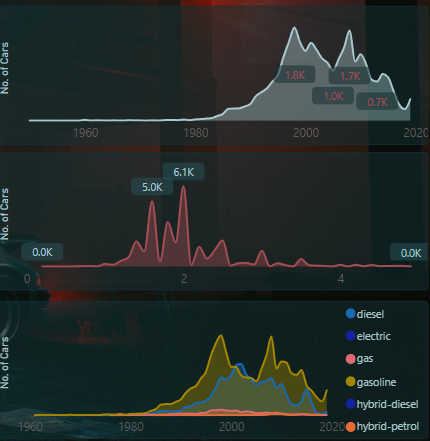
\includegraphics[width=0.6\textwidth]{Figures/PowerBI/areaplot.png}\\
  \caption{AreaPlots in PowerBI}
  \vspace{0.3cm}
\end{figure}
\\

\\
\subsubsection{Line Plots:}
Line plots are versatile visualizations for depicting trends and patterns in data over time or across different variables. They are commonly used to visualize time-series data, showing how a particular variable changes over a continuous period. Line plots are effective for identifying trends, detecting seasonality, and highlighting patterns such as upward or downward trends, oscillations, and outliers. For example, line plots can be used to visualize stock prices over time, temperature variations throughout the year, or sales trends for a particular product.

\subsubsection{Pie Charts:}
Pie charts are circular visualizations that represent categorical data as slices of a pie. Each slice corresponds to a category, and its size represents the proportion of that category relative to the whole. Pie charts are useful for showing the distribution of categorical data and highlighting the relative importance or contribution of each category to the total. They are commonly used in business presentations, marketing reports, and financial statements to visualize proportions, such as market share, budget allocations, or demographic distributions.

\\
\begin{figure}[htbp]
  \centering
  \vspace{0.3cm}
  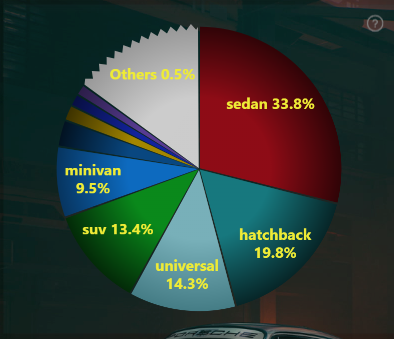
\includegraphics[width=0.6\textwidth]{Figures/PowerBI/piechart.png}\\
  \caption{PieChart in PowerB}
  \vspace{0.3cm}
\end{figure}
\\
\newpage
\subsubsection{Metric Cards:}
Metric cards provide a concise and focused representation of key performance indicators (KPIs) or summary statistics. They typically display a single value or metric along with contextual information such as a trend indicator, comparison to a target or benchmark, or historical performance. Metric cards are effective for providing at-a-glance insights and tracking progress towards goals or objectives. For example, a metric card might display the current sales revenue for a company along with a trend arrow indicating whether sales are increasing or decreasing compared to the previous period.

\subsubsection{Animated Bar Graphs:}
Animated bar graphs add a dynamic element to traditional bar charts by animating transitions between different states or time periods. They are useful for visualizing changes over time or comparing multiple variables across different categories. Animated bar graphs can enhance engagement and comprehension by highlighting temporal or sequential patterns in the data. For example, an animated bar graph might visualize monthly sales performance for different product categories over the course of a year, with each bar representing a month and the animation showing how sales patterns evolve over time.

\\
\begin{figure}[htbp]
  \centering
  \vspace{0.3cm}
  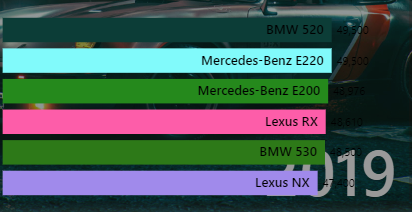
\includegraphics[width=0.8\textwidth]{Figures/PowerBI/animated barchart.png}\\
  \caption{Animated BarGraph in PowerBI}
  \vspace{0.3cm}
\end{figure}
\\

\\
\\
\newpage
\subsubsection{Doughnut Charts:}
Doughnut charts are similar to pie charts but feature a hole in the center, allowing for additional information or annotations to be displayed. They are useful for presenting categorical data in a compact and visually appealing manner, particularly when there are multiple categories or subcategories to visualize. Doughnut charts can convey the same information as pie charts while offering space for additional context or supplementary data. For example, a doughnut chart might visualize the distribution of expenses in a budget, with the outer ring showing high-level categories (e.g., housing, transportation, food) and the inner ring providing more detailed subcategories (e.g., rent, mortgage, utilities).
\\
\begin{figure}[htbp]
  \centering
  \vspace{0.3cm}
  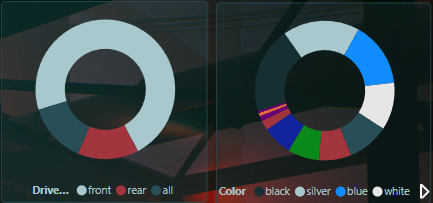
\includegraphics[width=0.7\textwidth]{Figures/PowerBI/doughnut.png}\\
  \caption{Doughnut Chart in PowerBI}
  \vspace{0.3cm}
\end{figure}
\\
}
\index{Dashboard Overview}


\newpage
\section{Results and Discussion}
\vspace{1cm}
{\fontsize{15}{15}\selectfont


\subsection*{Most Sold Car Brand: Volkswagen}
The analysis reveals that Volkswagen emerges as the most sold car brand, indicating its popularity and market dominance. This finding underscores Volkswagen's strong brand presence and consumer appeal, reflecting factors such as reliability, affordability, and innovative features. The significant market share captured by Volkswagen highlights its competitive advantage in the automotive industry.

\subsection*{Highest Priced Car: \textdollar50,000}
The dataset identifies a car priced at \textdollar50,000 as the highest-priced vehicle, reflecting the presence of premium or luxury cars in the market. This observation suggests the existence of diverse market segments catering to varying consumer preferences and purchasing power. The presence of high-end vehicles underscores the demand for luxury and performance-oriented automobiles, catering to affluent consumers seeking exclusivity and sophistication.

\subsection*{Number of Car Models Till 2019: 1,105}
The analysis indicates the existence of 1,105 unique car models in the USA up to the year 2019. This extensive variety underscores the diversity and innovation prevalent in the automotive industry, catering to diverse consumer needs and preferences. The abundance of car models reflects manufacturers' efforts to continually introduce new models, upgrade existing ones, and adapt to changing market trends, ensuring competitiveness and relevance in the dynamic automotive landscape.

\subsection*{Fuel Usage Preference: gasoline (petrol)}
The data highlights gasoline (petrol) as the predominant fuel choice among cars, indicating its widespread usage and availability. This preference for gasoline-powered vehicles aligns with historical trends and infrastructure development, where gasoline remains the primary fuel source for automobiles globally. Factors such as affordability, infrastructure support, and technological advancements contribute to gasoline's continued dominance in the automotive sector.
\newpage
\subsection*{Most Popular Car in 2019: BMW 520}
The analysis identifies the BMW 520 as the most popular car in 2019, reflecting its strong market presence and consumer appeal. This finding underscores BMW's reputation for producing high-quality, performance-oriented vehicles known for their luxury, comfort, and cutting-edge technology. The popularity of the BMW 520 in 2019 may be attributed to factors such as brand loyalty, product innovation, and effective marketing strategies, positioning it as a top choice among consumers in the competitive automotive market.

In summary, the results of the analysis provide valuable insights into various aspects of the automotive industry, including brand preference, pricing dynamics, market trends, and consumer behavior. Understanding these findings is essential for industry stakeholders, including manufacturers, policymakers, and consumers, to make informed decisions, drive innovation, and shape the future of the automotive sector.

}
\index{Results and Discussion}


\newpage
\section{Conclusion}
\vspace{1cm}
{\fontsize{15}{15}\selectfont

In conclusion, the analysis of the automotive data reveals several noteworthy trends and insights that shed light on the dynamics of the industry. Firstly, Volkswagen emerges as the most sold car brand, indicating its significant market share and widespread consumer acceptance. This underscores Volkswagen's strong brand reputation and competitive position in the automotive market. Secondly, the presence of a car priced at \text{\$}50,000 signifies the existence of premium offerings catering to affluent consumers seeking luxury and exclusivity. This reflects the diversity of the automotive market and the presence of distinct market segments with varying price sensitivities. Additionally, the dataset highlights the extensive variety within the automotive landscape, with a total of 1,105 unique car models identified in the USA until 2019. This underscores the industry's commitment to innovation and product diversity, catering to diverse consumer preferences and needs. Furthermore, the prevalence of gasoline as the primary fuel choice among cars underscores the continued dominance of conventional fuel sources despite the emergence of alternative technologies. Lastly, the BMW 520 emerges as the most popular car in 2019, showcasing the brand's appeal and strong market presence. This finding underscores the importance of brand reputation, product quality, and consumer perception in driving purchasing decisions within the automotive sector. Overall, these insights provide valuable information for industry stakeholders, enabling them to better understand market dynamics, consumer preferences, and emerging trends, ultimately guiding strategic decision-making and future developments in the automotive industry.
\\
\\
In addition to the compelling insights gleaned from the data, this analysis underscores the success of the data analysis methodology employed. Through meticulous data collection, preprocessing, and analysis, significant patterns and trends within the automotive industry have been uncovered. The systematic approach to exploring variables such as car brand sales, pricing dynamics, fuel preferences, and popular models has yielded comprehensive insights that contribute to a deeper understanding of the market landscape.
\\
\\
In essence, the successful outcome of this data analysis work underscores the importance of rigorous methodology, technical proficiency, and interpretive skill in extracting actionable insights from data. As a result, the findings presented not only enrich our understanding of the automotive industry but also showcase the efficacy of data-driven decision-making in driving strategic outcomes.
}
\index{Conclusion}


\newpage
\section{References}
\vspace{1cm}
{\fontsize{15}{15}\selectfont
\subsection{Internet :}
\vspace{0.6cm}
Dataquest. (2020). Introduction to Seaborn: A Brief Overview.\\
\href{https://www.dataquest.io/blog/seaborn-tutorial/}{https://www.dataquest.io/blog/seaborn-tutorial/}
\\
\\
Jupyter. (2024). Matplotlib: Visualization with Python.\\
\href{https://jupyter.org/documentation/interactive/magics.html#magic-matplotlib}{https://jupyter.org/documentation/interactive/magics.html#magic-matplotlib}
\\
\\
Kaggle. (2020). Car Features and MSRP.\\
\href{https://www.kaggle.com/CooperUnion/cardataset}{https://www.kaggle.com/CooperUnion/cardataset}
\\
\\
Pandas. (2024). pandas.DataFrame.describe.\\
\href{https://pandas.pydata.org/docs/reference/api/pandas.DataFrame.describe.html}{https://pandas.pydata.org/docs/reference/api/pandas.DataFrame.describe.html}
\\
\\
Seaborn. (2019). seaborn.lineplot.\\
\href{https://seaborn.pydata.org/generated/seaborn.lineplot.html}{https://seaborn.pydata.org/generated/seaborn.lineplot.html}
\\
\\
Source. (2024).Drive@Mayborg.\\
\href{https://drive.google.com/drive/folders/1XuJvwWx2dHc8vPEcNj69LvxAT8j8lfdt?usp=sharing}{Go to Source file : https://drive.google.com/drive/}\\
1XuJvwWx2dHc8vPEcNj69LvxAT8j8lfdt?usp=sharing
\\
\\ 
\subsection{Books :}
\vspace{0.6cm}

\begin{enumerate}
    \item "Python for Data Analysis" by Wes McKinney.\\
    \item "Data Analysis Using SQL and Excel" by Gordon S. Linoff and Daniel T. Berry\\
    \item "Data Visualization: A Practical Introduction" by Kieran Healy\\
    \item "Hands-On Machine Learning with Scikit-Learn, Keras, and TensorFlow" by Aurélien Géron
\end{enumerate}

}
\index{References}

\end{document}